\documentclass{article}
\usepackage[UTF8]{ctex}  % 使用中文支持包
\usepackage[a4paper, margin=1in]{geometry}  % 设置纸张大小和边距
\usepackage{anyfontsize}  % 解决字体大小报错问题
\usepackage{fancyhdr}  % 设置页眉、页脚、页码
\usepackage{lscape}
\usepackage{longtable}  % 支持长表格
\usepackage{booktabs}
\usepackage{graphicx}
\usepackage{colortbl}
\usepackage{tabularx}
\usepackage{multirow}
\usepackage[table,xcdraw]{xcolor}

\usepackage{amsmath}  % 数学公式支持
\usepackage{cases}  % 支持联立编号
\usepackage[sort]{natbib}  %国标参考文献 with sorting option

\usepackage{graphicx}  % 插入图片支持
\usepackage{float}  % 设置图片浮动位置
\usepackage{subfigure}  % 插入多图时用子图显示

\usepackage{abstract}

\usepackage{listings}  % 代码块支持
\usepackage{xcolor}  % 设置代码块颜色

\lstset{
    basicstyle          =   \sffamily,          % 基本代码风格
    keywordstyle        =   \bfseries,          % 关键字风格
    commentstyle        =   \rmfamily\itshape,  % 注释的风格,斜体
    stringstyle         =   \ttfamily,  % 字符串风格
    flexiblecolumns,                % 别问为什么,加上这个
    numbers             =   left,   % 行号的位置在左边
    showspaces          =   false,  % 是否显示空格,显示了有点乱,所以不现实了
    numberstyle         =   \zihao{-5}\ttfamily,    % 行号的样式,小五号,tt等宽字体
    showstringspaces    =   false,
    captionpos          =   t,      % 这段代码的名字所呈现的位置,t指的是top上面
    frame               =   lrtb,   % 显示边框
}

\lstdefinestyle{Python}{
    language        =   Python, % 语言选Python
    basicstyle      =   \zihao{-5}\ttfamily,
    numberstyle     =   \zihao{-5}\ttfamily,
    keywordstyle    =   \color{blue},
    keywordstyle    =   [2] \color{teal},
    stringstyle     =   \color{magenta},
    commentstyle    =   \color{red}\ttfamily,
    breaklines      =   true,   % 自动换行,建议不要写太长的行
    columns         =   fixed,  % 如果不加这一句,字间距就不固定,很丑,必须加
    basewidth       =   0.5em,
}

\usepackage[hyphens]{url}  % 支持链接换行
\usepackage{hyperref}  % 超链接支持

\hypersetup{
    hidelinks,
    colorlinks=true,
    allcolors=black,
	pdfstartview=Fit,
	breaklinks=true
}

\usepackage{gbt7714}  %国标参考文献

\bibliographystyle{gbt7714-numerical}

\usepackage{lastpage}  % 添加lastpage包

\newcommand\f[2]{\frac{#1}{#2}}
\newcommand\pf[2]{\frac{\partial#1}{\partial#2}}
\newcommand\df[2]{\dfrac{#1}{#2}}
\newcommand\pdf[2]{\dfrac{\partial#1}{\partial#2}}
\newcommand\zsin[1]{\frac{e^{i#1}-e^{-i#1}}{2i}}
\newcommand\zdsin[1]{\dfrac{e^{i#1}-e^{-i#1}}{2i}}
\newcommand\zcos[1]{\frac{e^{i#1}+e^{-i#1}}{2i}}
\newcommand\zdcos[1]{\dfrac{e^{i#1}+e^{-i#1}}{2i}}
\newcommand\zline[1]{#1-\overline{#1}}
\newcommand\dg[2]{#1^{\circ}#2'}

\setlength{\headheight}{16pt}
\pagestyle{fancy}
\fancyhf{}

\title{\bf\huge 自然循环工作原理}
\author{Jerry}
\date{\today}
\pagenumbering{arabic}

\begin{document}

\fancyhead[L]{Jerry}
\fancyhead[C]{自然循环工作原理}
\fancyhead[R]{核电厂系统与设备-黄善仿}
\fancyfoot[C]{\thepage}

\maketitle
\tableofcontents

\begin{abstract}
    自然循环是一种基于流体密度差驱动的被动冷却机制,广泛应用于核反应堆、太阳能热水器、发电厂及电子设备等领域。其原理源于流体热膨胀和冷缩特性,形成不依赖外部动力的循环流动。自然循环可分为单相和两相流动,性能受系统设计、热源与冷源的温差、流体性质及外部环境等多种因素影响。在核反应堆中,自然循环被广泛用于紧急停堆及断电条件下移除衰变热,提升安全性和可靠性。本文总结了自然循环的基本原理、主要影响因素及核电厂设计中的应用实例,为工程设计提供参考。
\end{abstract}

\textbf{关键词:} 自然循环;核反应堆;被动冷却;安全性;可靠性

\section{自然循环(Natural Circulation)}

自然循环是一种基于流体密度差异驱动流动的机制,广泛应用于核反应堆冷却、太阳能系统、地热能利用以及电子设备散热等领域。在自然循环系统中,流体通过热源与冷源之间的温差发生密度变化,由此产生的密度差驱动流体循环,实现热量的传递与分布。

\subsection{自然循环的基本原理}

如图\ref{fig:cold-warm},自然循环的核心原理源于流体的热膨胀和冷缩特性。当流体被热源加热时,其温度升高,体积膨胀,密度减小,变得比周围的冷流体轻。在重力作用下,这部分低密度流体向上移动。到达冷源处后,流体失去热量,温度降低,密度增加,变得比周围的热流体重,进而向下流动,形成一个持续的循环。

\begin{figure}[htbp]
    \centering
    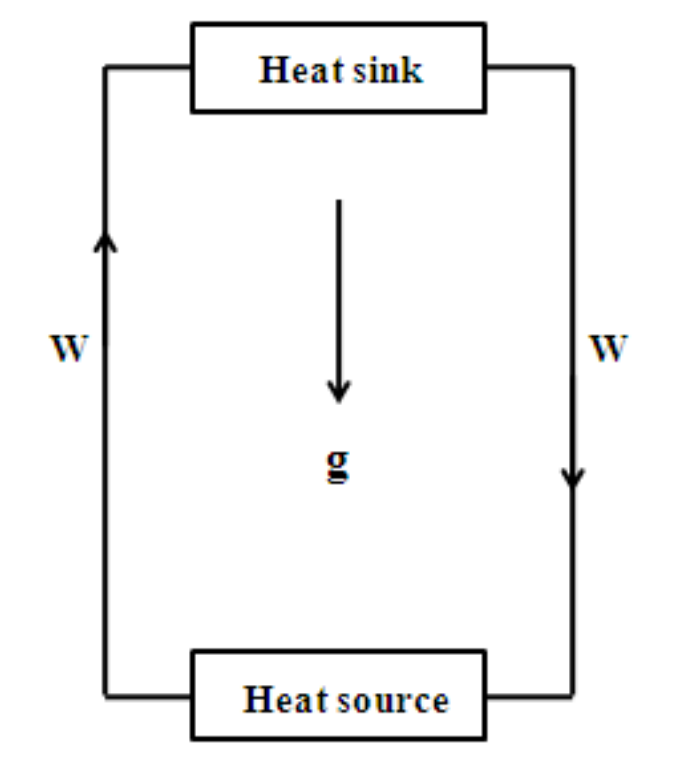
\includegraphics[width=0.2\textwidth]{figures/cold-warm.png}
    \caption{自然循环示意图}
    \label{fig:cold-warm}
\end{figure}

这种流动的驱动力来自温差引起的密度差,具体表现为浮力压差。在重力场或类似的力场中,这种密度梯度会自然产生流体的循环流动。自然循环的过程无需任何外部动力设备,比如泵\cite{thakuriaINVESTIGATIONSSUBCRITICALSUPERCRITICAL}。

根据流体的相态变化,自然循环可分为单相和两相两种形式。单相自然循环指流体在循环过程中始终保持单一相态,例如液态水在整个系统中流动而不发生相变。\cite{reventosParametersConcepts2017a}而两相自然循环则涉及流体在循环中经历相态变化,如液体在热源处沸腾形成气体,或气体在冷源处凝结成液体。这种相变过程能够显著提高传热效率和循环能力,但也对系统的设计和控制提出了更高的要求。

自然循环的性能受多种因素的综合影响。首先,热源与冷源之间的温差是驱动循环的核心,温差越大,产生的密度差越明显,从而驱动力更强。其次,系统的几何结构至关重要,包括管道的布置方式、热源与冷源的相对位置以及两者之间的高度差,这些都会直接影响流体流动的效率。此外,流体本身的物理性质,例如密度、粘度、比热和导热系数等,也会显著影响循环性能。操作条件同样不可忽视,例如系统内的压力水平和加热功率大小等参数会对流动状态产生调节作用。最后,外部环境中的因素,例如海洋环境中的摇摆或振动等动态条件,也可能对自然循环的稳定性产生重要影响。\cite{aksanTargetPhenomenaNuclear2017a}

\subsection{自然循环的优点}

自然循环作为一种高效的被动冷却机制,在许多工程领域都有重要应用,尤其是在对安全性和可靠性要求极高的场合。因此,自然循环的应用范围十分广泛,涵盖了多个关键领域。例如,在核反应堆中,自然循环被用于在紧急停堆或断电情况下移除堆芯的衰变热,从而保障反应堆的安全运行。在太阳能热水器中,自然循环有效地将太阳吸收的热能传递至水箱,为日常生活提供热水支持。此外,在化石燃料发电厂,自然循环锅炉通过高效传热实现能量转换,而热虹吸管则是工业中常见的自然循环装置之一。最后,在电力传输设备中,自然循环被用于变压器冷却,帮助维持设备的运行效率并延长其使用寿命。

与依赖泵的主动循环系统相比,自然循环系统具备显著的优势。首先,它不需要泵等外部动力设备,因而减少了对电力供应和相关辅助系统(如润滑、冷却和密封系统)的依赖,从而实现了更简单的设计。其次,由于系统中没有复杂的活动部件,其故障率显著降低,可靠性更高。此外,自然循环系统在失去动力的情况下仍然能够正常工作,尤其是在核反应堆等关键系统中,可以有效移除热量并保障安全运行,从而体现出更高的安全性。

\section{核电厂设计中的自然循环}

核反应堆即使在关闭后,由于裂变产物的放射性衰变,仍会持续产生热量。这种衰变热如果得不到有效冷却,可能会导致燃料过热,甚至熔化。比如在福岛核电站事故中,大地震和随后的海啸引发了长期断电,最终导致燃料损坏。

为应对这种情况,核反应堆通常设计了自然循环冷却系统。自然循环基于流体力学和热力学的基本物理定律,可以在无外部动力的情况下自动将衰变热带走。由于自然循环依赖系统本身的结构和物理性质,故障率较低。只要存在热源(燃料)和热汇(冷却系统),自然循环便能持续运行。因此,几乎所有核反应堆的设计都致力于在完全失去动力(CLOP)的情况下,通过自然循环有效移除衰变热,以确保堆芯安全。

\subsection{一些自然循环系统的例子}

\subsubsection{升高的水箱自然循环回路(堆芯补水水箱)}

自然循环回路是一种有效的堆芯冷却手段。如图\ref{fig:upward-tank}所示,一些先进反应堆设计中,在堆芯容器的顶部和底部连接有高架水箱,这些水箱通过管线与反应堆容器或主回路相连。水箱内通常注满硼水,以便在系统压力作用下为反应堆提供冷却剂。为了实现功能控制,水箱通过底部排放管线上的隔离阀与反应堆容器隔离,而顶部连接管线则用于感应整个系统的压力。

在紧急情况下,通过打开底部隔离阀,可以完成自然循环回路,使硼水流入堆芯,为其提供冷却。这一设计中,为了减少与反应堆压力容器相连的管线数量,堆芯补水箱(CMT)的输送管线通常与堆芯紧急冷却剂输送管线共用。

在多种事故工况下,CMT输送可能会在蓄水池供水启动之前开始,并在蓄水池排空后停止。在此过程中,CMT的流量可能会受到蓄能器流量的显著影响。此外,特别是当CMT输送管线连接至冷却回路或热管(即不直接向容器内部喷注冷却剂时),需要检查排放管线中流体的流动方向。换言之,CMT的冷却液可能用于冷却蒸汽发生器,或者在某些情况下偏离其核心冷却的主要任务。\cite{international2009iaea}

\begin{figure}[htbp]
    \centering
    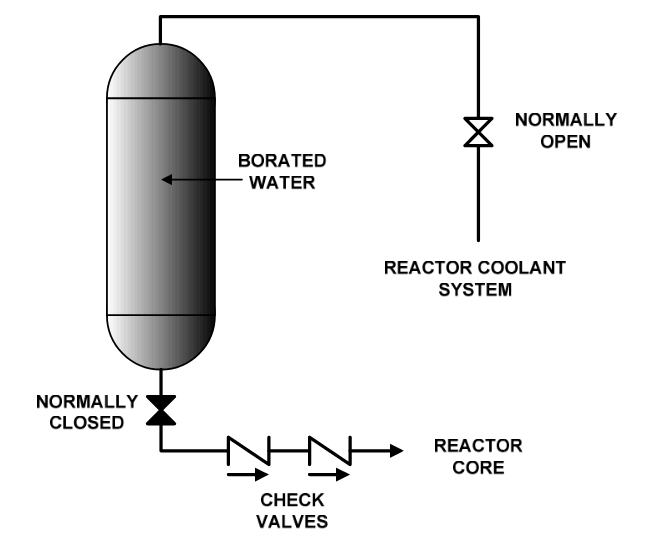
\includegraphics[width=0.3\textwidth]{figures/upward-tank.png}
    \caption{升高的水箱自然循环回路}
    \label{fig:upward-tank}
\end{figure}

\subsubsection{高处的水槽或水箱}

在低压条件下,装有冷硼酸水的高架水箱可以利用重力作用为堆芯提供冷却水,将堆芯淹没。在某些设计中,水箱的容量足以填满整个反应堆腔。如图\ref{fig:high-tank}所示,该系统的运行依赖于打开隔离阀,同时确保流体的驱动压头超过系统压力加上止回阀的开启压力。在堆芯暴露的情况下,由于堆芯区域产生蒸汽,可能会对重力排水箱的性能造成一定限制。\cite{international2009iaea}

\begin{figure}[htbp]
    \centering
    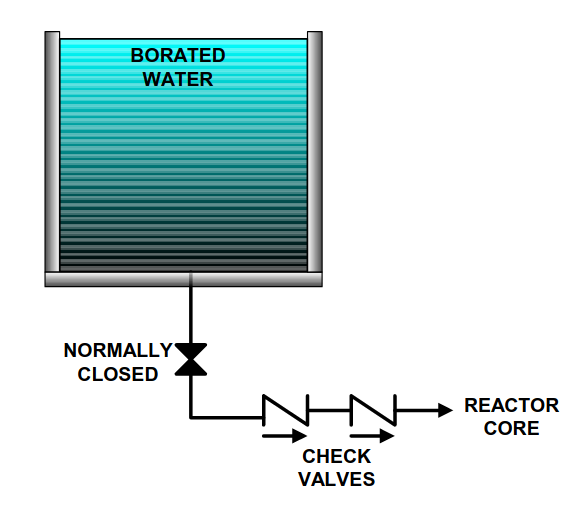
\includegraphics[width=0.3\textwidth]{figures/high-tank.png}
    \caption{高处的水槽或水箱}
    \label{fig:high-tank}
\end{figure}

\subsubsection{被动冷却蒸汽发生器自然循环}

此外,一些先进压水堆设计集成了通过蒸汽发生器被动移除衰变热的系统。具体而言,蒸汽发生器产生的蒸汽在浸没于水箱中的热交换器或空气冷却系统中冷凝,如图\ref{fig:steam-generator}所示。该系统通过热交换器将蒸汽发生器的热量传递至水箱,使水箱中的水沸腾并产生蒸汽。生成的蒸汽通过自然对流进入蒸汽发生器,形成一个闭合的自然循环,有效移除衰变热。这一设计进一步提高了系统的安全性和被动冷却能力。\cite{khanNuclearPowerPlant2020a}

\begin{figure}[htbp]
    \centering
    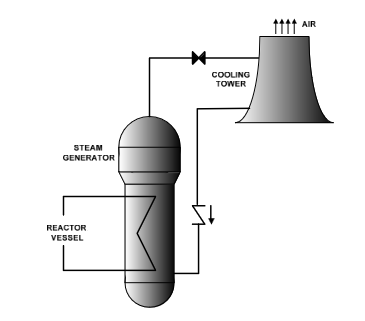
\includegraphics[width=0.3\textwidth]{figures/steam-generator.png}
    \caption{被动冷却蒸汽发生器自然循环}
    \label{fig:steam-generator}
\end{figure}

\subsubsection{自然循环的贮液槽}

此外,一些反应堆设计利用反应堆腔体及安全壳下部作为冷却剂储存器,在主回路失效时为堆芯提供冷却水。当反应堆系统损失的水被收集至安全壳贮水池后,最终将反应堆完全淹没,并通过打开隔离阀实现冷却水循环。堆芯中的水沸腾后,带走衰变热,产生的蒸汽通过自动减压系统(ADS)阀向上排放至安全壳内。如图\ref{fig:liquid-tank}所示,堆芯区域与贮水池之间的密度差产生了自然循环流动,水通过贮水池滤网进入反应堆容器,足以带走衰变热。在某些设计中,反应堆容器内部的自然循环本身就足以移除衰变热,无需ADS运行支持。\cite{international2009iaea}

\begin{figure}[htbp]
    \centering
    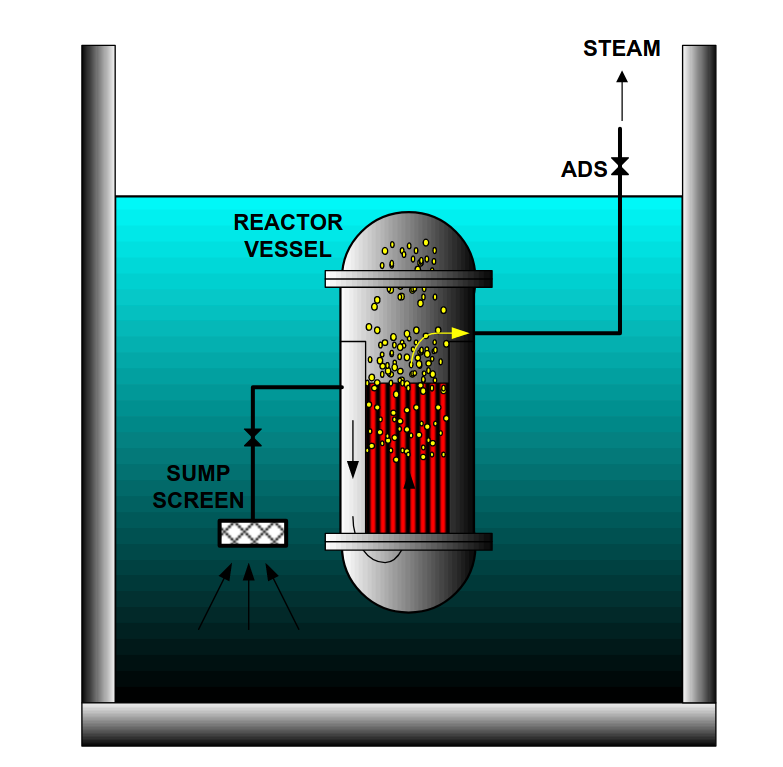
\includegraphics[width=0.3\textwidth]{figures/liquid-tank.png}
    \caption{自然循环的贮液槽}
    \label{fig:liquid-tank}
\end{figure}

\bibliography{cite.bib}

\begin{abstract}
    Natural circulation is a passive cooling mechanism driven by fluid density differences and finds extensive applications in nuclear reactors, solar water heaters, power plants, and electronic systems. It operates based on the thermal expansion and contraction of fluids, enabling circulation without external power. Natural circulation can be categorized into single-phase and two-phase flows, with performance influenced by system design, temperature gradients, fluid properties, and environmental factors. In nuclear reactors, natural circulation is employed to remove decay heat under shutdown and power-loss scenarios, enhancing safety and reliability. This paper reviews the fundamental principles, key influencing factors, and application examples of natural circulation in nuclear power plant designs, providing insights for engineering practices.
\end{abstract}

\textbf{Keywords:} Natural circulation, nuclear reactors, passive cooling, safety, reliability

\end{document}